\chapter{Anforderungen und Konzept}
Das Thema der Bachelorarbeit \textit{\glqq Entwicklung einer webbasierten Applikation zur Bearbeitung von PDF Dateien\grqq} habe ich selbst gewählt. Ziel der Arbeit ist eine PDF-Webapplikation zu entwickeln, die gängige Funktionalitäten, die man bei üblicher PDF-Bearbeitung benötigt, bieten soll. Gängige Funktionalitäten sind für mich ein PDF-Reader, das Editieren von Seiten und die grundsätzlichsten Grafikoperationen. Mir war außerdem wichtig, dass die PDF Web App auf allen Desktop-Plattformen Windows, macOS und Linux einsetzbar ist, da PDF genauso ein plattformunabhängiges und hardwareunabhängiges Format ist. Ich habe mir selbst die Vorgabe gestellt, dass die PDF Web App lediglich als Desktop-App funktionieren muss und nicht optimiert für Tablet oder Smartphone sein soll. PDF-Bearbeitung macht für mich am meisten Sinn in einer Desktopumgebung, da der Bildschirmabmessungen auf Tablets und vor allem bei Smartphones nicht besonders groß bis sehr klein ist. PDF-Bearbeitung nimmt viel Zeit in Anspruch und am besten setzt man sich an den Schreibtisch vor einen großen Bildschirm und setzt seine PDF-Modifikationen mit der Maus und Tastatur um. \\
Ursprünglich war die PDF Web App als offline Webseite angedacht. Die Webseite sollte man auch ohne Internetverbindung wie ein Programm verwenden können, nur dass keine Installation notwendig ist. Das einzige Programm, was man benötigt für die Ausführung der PDF Web App soll ein Browser sein. Durch Öffnen der index.html im Browser kann man die PDF Webapp auf einfache Art und Weise starten und benutzen. Eine Anforderung an mich selbst ist, dass sie als Open Source-Projekt für jeden kostenlos nutzbar sein soll, da ich selbst nur kostenlose PDF-Bearbeitungsprogramme verwende. So soll die PDF Web App auch u.a. für Studenten mit wenig Geld zur Verfügung stehen. Das Open Source-Projekt soll als öffentliches Repository auf Github vorhanden sein und jeder kann es downloaden. Da das PDF-Dateiformat ein offenes Dateiformat ist, bin ich der Ansicht, dass die Bearbeitungsprogramme für PDF-Dateien ebenfalls kostenlos sein sollten. Auf dem öffentlichen Github Repository soll man ausschließlich die PDF Web App mit Tutorials und einer Beschreibung ohne Werbeprogramme oder ähnliches herunterladen können. \\
Des Weiteren wollte ich mich nur auf HTML, CSS und JavaScript beschränken. Folglich ist die PDF Web App eine reine Frontend Web Anwendung und ich wollte kein Backend oder eine Datenbank implementieren. Dadurch habe ich die Programmierung und den Verwaltungsaufwand meiner PDF Web App simpler gemacht. Die Bedienung sollte möglichst intuitiv, eingängig und einfach gehalten sein, damit ein Nutzer nicht seitenlange Tutorials lesen muss. In der Praxis bedeutet das, dass die Einstellmöglichkeiten möglichst durch reines Ausprobieren erfasst werden können. Um diese Anforderung zu erreichen, sollte eine GUI mit simplem, übersichtlichem und strukturiertem Design verwendet werden. Verschlüsselung wollte ich Außerachtlassen, da das PDF-Dateiformat unsicher ist und generell nicht für vertrauliche Inhalte verwendet werden sollten. Formulare und Kommentare, sowie das incremental update wollte ich ebenfalls nicht implementieren, um den Arbeitsaufwand geringer zu halten und weil ich diese Anwendungsgebiete kaum verwende. Ich wollte mich lediglich auf die wichtigsten Funktionen zur Bearbeitung beschränken.


\subsection{Vorgaben für den Funktionsumfang der PDF Web App}
Bei der Planung der PDF Web App habe ich den Funktionsumfang selbstständig zusammengestellt. Im Prinzip sollte die PDF Web App aus 8 Modulen bestehen, wobei die letzten 4 Module in der Liste den Editor bilden:

\begin{itemize}
	\item Reader
	\item Creator
	\item Merger
	\item Splitter
	\item Writer
	\item Drawer
	\item Geometry Editor
	\item Images Editor
\end{itemize}

Im Editor sollen die aktuellen Koordinaten des Mauscursors angezeigt werden. Der Reader sollte eine Navigationseinheit enthalten, die die aktuelle Seitenzahl anzeigt, zu einer beliebigen Seite springen kann, eine Zoomfunktionalität implementiert und zur vorherigen und nächsten Seite blättern kann. Zusätzlich soll eine Druckfunktionalität enthalten sein. Der Creator ist ein Modul zur Erstellung von leeren PDF-Dokumenten als Download mit beliebiger Größe, Anzahl an Seiten, Möglichkeiten, die Orientierung (Portrait, Landscape, quadratisch), zu justieren und Presets zur DIN A Größe. Es gibt 2 Module zur Verwaltung von kombinierten PDF-Dokumenten. Zum einen soll der Merger mehrere PDF-Dateien zusammenfügen und als eine Datei speichern können. Dabei soll die Reihenfolge der einzelnen PDF-Dateien in einer Liste anpassbar sein und eine Druckfunktion enthalten. Hingegen soll der Splitter ein PDF zerteilen und als einzelne PDF-Dateien speichern können. Dabei gibt es verschiedene Split-Operationen: Der Splitter soll nach jeder, nach jeder ungeraden, nach jeder geraden, nach einer bestimmten und nach einer Liste an Seiten das PDF zerteilen können. In meiner PDF Web App ist Speichern ein Synonym für den Download eines bearbeiteten PDFs. Beim Download soll man immer einen benutzerdefinierten Dateinamen setzen können. Diese 4 Module sind im Diagramm \ref{fig:modules4} graphisch dargestellt. 

\begin{figure}[!htbp]
	\centering
	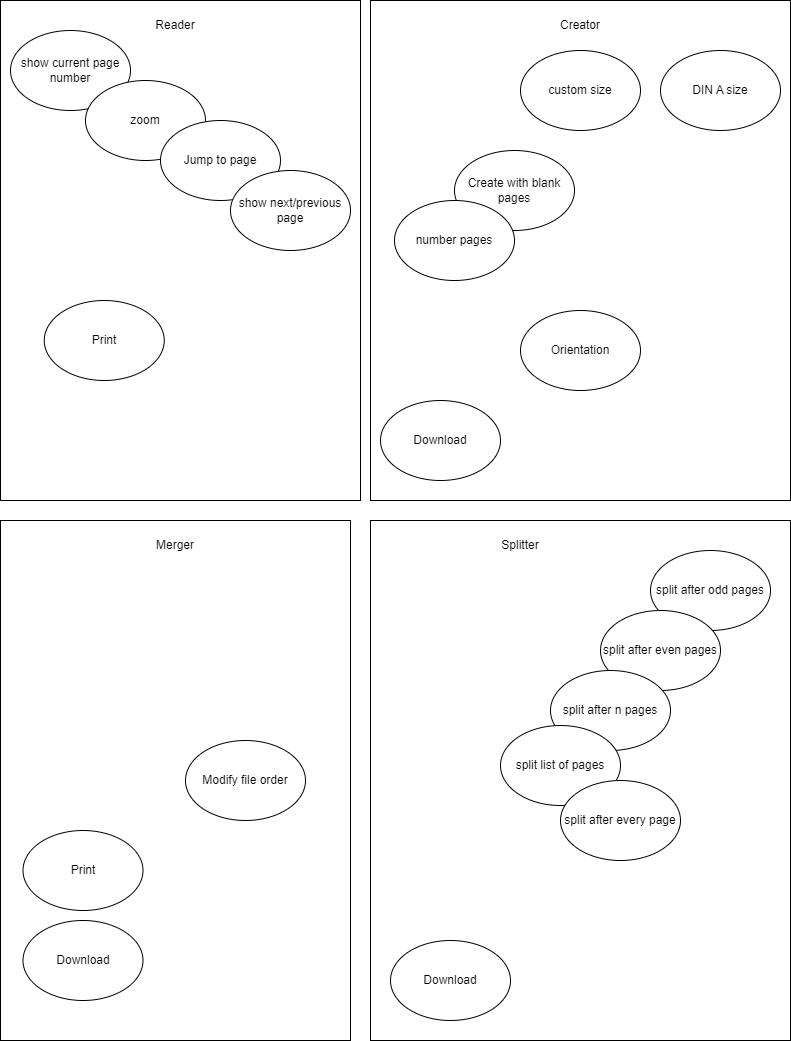
\includegraphics[width=0.9\textwidth]{"images/app-funktionen-anforderungen.png"}
	\caption{Anforderungen an den Reader, Creator, Merger und Splitter der PDF Web App}
	\label{fig:modules4}
\end{figure}

Der Editor besteht aus den restlichen 4 Modulen. Alle Editoroperationen beziehen sich lediglich auf bereits hinzugefügte Elemente. Es sollen keine schon im geöffneten PDF bestehende Objekte bearbeitet werden können. In jedem Editorteil soll es möglich sein, zu drucken und das PDF zu downloaden, sowie alle neuen Elemente auf einen Schlag zu löschen. Außerdem sollen Elemente in beliebiger Reihenfolge übereinander stapelbar sein, d.h. man kann Elemente in den Vordergrund holen oder weiter nach hinten Richtung Hintergrund verschieben. Im Diagramm \ref{fig:editor}, was zeigt, wie die Editormodule aufgebaut sind, ist die zuletzt genannte Funktionalität mit z-axis order gekennzeichnet. Mittels des Writers soll Text hinzugefügt werden können. Dieser neue Text kann gelöscht, verschoben, gedreht, die Schriftgröße und font family angepasst und eingefärbt werden. Als Font kann man zwischen Times Roman, Helvetic oder Courrir und dessen Schriftschnitten wählen bzw. einen benutzerdefinierten Font verwenden. Im Drawer hat man die Möglichkeit zu zeichnen und zu radieren. Dabei kann man die Größe und Farbe des Stifts bzw. Radierers anpassen. Das Geometry Editor-Modul soll geometrische Formen, wie Rechteck, Dreieck oder Ellipse hinzufügen, ihre Größe und Farbe verändern, Formen löschen, verschieben und drehen können. Zuletzt soll der Images Editor Bilder vom Dateisystem hinzufügen, löschen, verschieben und drehen können.


\begin{figure}[!htbp]
	\centering
	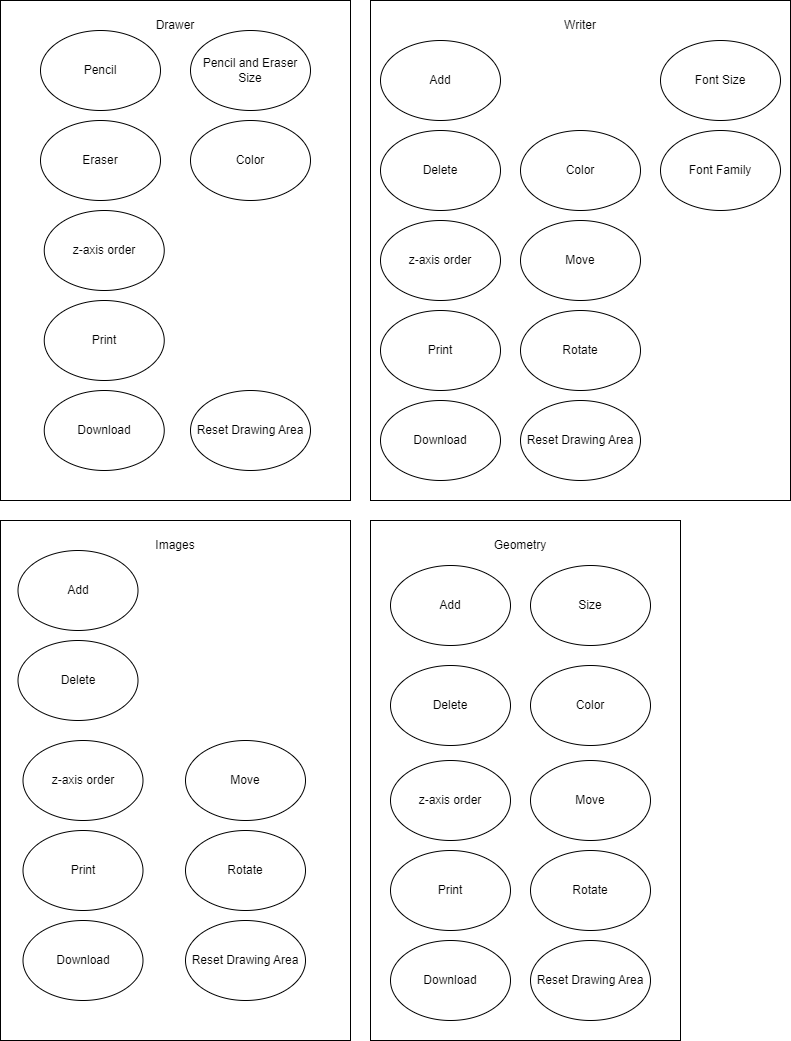
\includegraphics[width=0.9\textwidth]{"images/editor-funktionen-anforderungen.png"}
	\caption{Anforderungen an den Editor der PDF Web App}
	\label{fig:editor}
\end{figure}


\subsection{Qualitätsanforderungen}
Ich habe den Ansporn, dass die PDF Web App sehr stabil und mit minimalen zeitlichen Verzögerungen arbeiten soll. Konkret bedeutet das, dass sich die Seite schnell aufbauen kann und die Seiten von geöffneten PDFs in einer akzeptablen Zeitspanne laden sollen. Genauso wichtig ist mir eine gute Funktionalität, d.h. keine Laufzeitfehler bzw. dass die PDF Web App immer genau gleich funktioniert und nicht abstürzt. Maximale Effizienz sollte gegeben sein, indem die PDF Web App als reine Frontend App ohne Backend auskommen kann. Es müssen keine Daten gespeichert werden bzw. muss sich der Benutzer nirgendwo registrieren und einloggen. Genauso wichtig ist eine gute Benutzbarkeit. Genauer gesagt soll der Anwender sich die Funktionalität der PDF Web App möglichst selbstständig durch Ausprobieren erschließen können. Die Beschriftung der Buttons sollte selbsterklärend sein und die Layoutfarben so eingesetzt, dass sie eine Designkonsistenz zur Vermittlung von Funktionalitätsgruppen aufweist. Die Änderbarkeit und Erweiterbarkeit sollte auf einfache Weise möglich sein, sodass auch andere Entwickler an der PDF Web App arbeiten können. Des Weiteren sollte die Portierbarkeit hoch sein, denn die PDF Web App muss auf den Desktop-Betriebssystemen Windows, macOS oder Linux immer gleich funktionieren. Eine Tablet- oder Mobilversion ist nicht geplant. Mir war wichtig, dass man die PDF Web App als Offlinewebseite im Browser verwenden kann, quasi wie ein eigenständiges Programm, was man nicht installieren muss. Alle gängigen Browser sollten die index.html-Datei der PDF Web App öffnen und ausführen können. Außerdem soll man ausschließlich die PDF Web App und eventuelle Tutorials bzw. eine Beschreibung auf Github downloaden können. Es sollen keine zusätzlichen Werbedateien oder -programme zum Download angeboten werden. Die wichtigste Bedingung, dass die PDF Web App ein kostenloses Open Source-Projekt sein soll, muss auch für zukünftige Releases und Updates, gültig bleiben. 